\chapter{SENSATION TACTILE}
Ici nous présentons le chemin de l’information et détaillons les points clé dans des sections séparé.\par

\section{Cheminement de l’information}
La zone 3b est seulement à 3 synapses de la fibre sensorielle. (via le cuneate nucleaus and the talamus).\par
\begin{figure}[!h]
	\centering
	\includegraphics[width=10cm]{1_Bible/Photos/Biology/chemin.jpg}
	\caption{Cheminement de l’information}\label{chemin_info}
\end{figure}

\section{Mécanique du contact}

\subsection{Définition des termes}
Force : Dans la mécanique du point, une force est représenté par une direction (vecteur) et une amplitude (scalaire). Dans la mécanique du solide, le concept est étendu à une matrice 3x3 où chaque ligne représente les forces soumises sur les faces du cube élémentaire. On parle alors de tenseur de force. Les éléments sur la diagonale du tenseur sont appelés les efforts normaux, et les autres les efforts tangentiels. Dans certain cas, une matrice du moment peut être définie pour décrire les forces de rotations.\par
Déformation : La différence de géométrie entre l’état l’initiale et l’état qui suit l’exercions  du tenseur de force peut être définie avec un tenseur de déformation.\par
Élasticité : Décris la capacité d’un matériau de résister une force qui lui est appliqué. Exprimé avec le coefficient de Young.\par
Viscosité : Décris la composante temporelle qui lie application d’une force et déformation.\par
Compressibilité : Décris la capacité d’un matériau à se comprimer. Exprimé avec le coefficient de poisson.\par

….Distinction entre force normale, pression ; glissement, effort tangentiel; contraint, effort; tenseur de déformation…\par
…Distinction entre force et pression\par

\subsection{Contact statique}
Loi de hooke : Relie les deux grandeurs force et déformation\par
Contact Hertzien : Décrie les déformations\par

\subsection{Contact dynammque}
...

\subsection{Déformation local}
...

\subsection{Déformation distante -- Propagation des ondes}
Lors d’un stimulus tactile, des ondes se propagent à la surface de la peau, dans les couches inférieures de la peau et dans les organes. De ce fait les MRs distant du point de contact sont aussi stimulé par le contact. En plus de MRs cutanée, les MRs au niveau des muscles, tendons et articulation sont aussi stimulé. Il a été mis en évidence, que selon l’interaction tactile, le motif de propagation d’ondes sera différent. Ce qui alimentent l’hypothèse que ces ondes sont pris en comptent lors de l’interprétation d’un stimulus. Par exemple, lors d’un toucher d’exploration, la texture de la surface va créer un motif d’ondes particulier qui se fera sentir jusqu’au poignet, où des PC récepteurs pourront encodé la texture et ainsi permettre l’indentification de la texture parcouru.\par

Qu’est ce qui est pondérant, la propagation de la vibration : dans la peau, dans les os, dans les tendons ?\par

\section{Mécano-transduction}
Sous la stimulation, les mécanorécepteurs émettent des potentiels d’action le long des nerfs afférents et en direction du CNS. Le procédé par lequel une excitation sensorielle (ici mécanique) donne lieu à un potentiel d’action est nommé mécano-transduction. Ce procédé a fait l’objet de différentes études et a été modélisé.\par
Chaque mécanorécepteur encode la déformation mécanique en un potentiel d’action d’une manière différente. Il est a noté aussi que chaque mécanorécepteur semble sensible à différents types de stimuli (voir correspondant sous-partie).\par

\subsection{PC}
...

\subsection{RA}
...

\subsection{SAI}
...

\subsection{SAII}
...

\subsection{Fibre de type C}
...

\subsection{Exemple de modélisation}
...

\section{Séquence de potentiel d’action (spike train)}
Les mécanorécepteurs produisent une séquence de potentiel d’action dont l’amplitude et la fréquence est propre à la caractéristique de la sensation. La séquence de potentiel d’action peut alors être interprété comme l’encodage de la sensation.\par
\begin{figure}[!h]
	\centering
	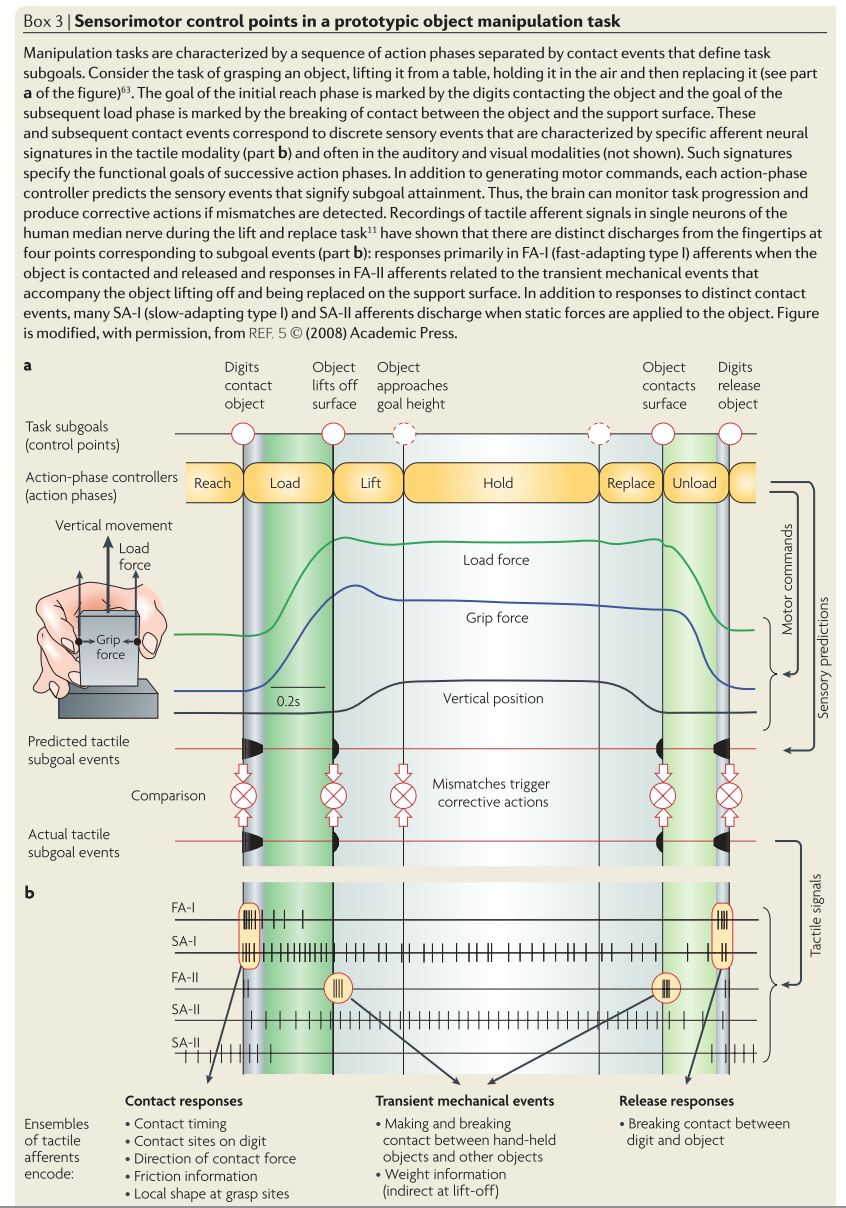
\includegraphics[width=12cm]{1_Bible/Photos/Biology/potentiel_daction.png}
	\caption{Exemple de séquence de potentiels d'action lors d'une tache de manipulation}\label{potentiel_daction}
\end{figure}

\section{Mesure Psychophysique}
Le sens du toucher peut sentir divers stimuli tactile. Néanmoins, comme tout récepteur/senseur, il ne peut sentir qu’à partir d’une intensité minimum (seuil de perception) et ne peux distinguer qu’une différence minimale entre deux intensités (seuil de discrimination). Ces caractéristiques peuvent être mesuré et quantifié grâce à divers expériences  psychophysiques (exemple tableau ci-dessous).\par
\begin{table}[!h]
	\caption{Seuil de perception (résolution) et seuil de discrimination (weber fraction) pour différent types de sensation (stimulus dimension)}
	\label{tab_mesure_psycho}
	\centering
	\begin{tabular}{|p{5cm}|p{5cm}|p{4cm}|}
		\hline \rule[-7pt]{0pt}{20pt}
		Dimension de la stimulation&Résolution&Fraction de Weber(\%)\\
		\hline
		\rule[-7pt]{0pt}{20pt}Texture de surface (rugosité)& 0.06... & 5-12\% \\
		\hline
		\rule[-7pt]{0pt}{20pt}...&...& ...\\
		\hline
		\rule[-7pt]{0pt}{20pt}...&...&...\\
		\hline 
		\rule[-7pt]{0pt}{20pt}...&...&...\\
		\hline
		\rule[-7pt]{0pt}{20pt}...&...& ...\\
		\hline
		\rule[-7pt]{0pt}{20pt}...&...&...\\
		\hline 
		\rule[-7pt]{0pt}{20pt}...&...&...\\
		\hline
		\rule[-7pt]{0pt}{20pt}...&...& ...\\
		\hline
		\rule[-7pt]{0pt}{20pt}...&...&...\\
		\hline 
		\rule[-7pt]{0pt}{20pt}...&...&...\\
		\hline
		\rule[-7pt]{0pt}{20pt}...&...& ...\\
		\hline
		\rule[-7pt]{0pt}{20pt}...&...&...\\
		\hline 
		\rule[-7pt]{0pt}{20pt}...&...&...\\
		\hline
		\rule[-7pt]{0pt}{20pt}...&...& ...\\
		\hline
		\rule[-7pt]{0pt}{20pt}...&...&...\\
		\hline
	\end{tabular}
\end{table}
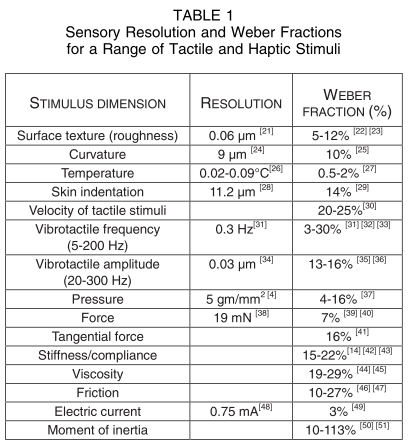
\includegraphics[width=10cm]{1_Bible/Photos/Biology/tab_seuil.png}

\subsection{Seuil de perception -- \textit{Threshold}}
...

\subsection{Seuil de discrimination -- \textit{JND}}
...

\subsubsection{Seuil de discrimination spatiale}
La méthode du seuil de discrimination spatiale consiste à déterminer la distance minimale qu’un sujet (les yeux fermés) n’arrive plus à distinguer les deux pointes qui lui appliqué sur la peau. En fonction des différentes partie du corps, le seuil – entre ressentir les deux pointes et le passage ou le sujet ne pense qu’il n’y en a plus qu’une. Zones plus sensible de que d’autre. Les MRs ne sont pas réparti de la façon sur le corps, la densité est différente.\par
\begin{figure}[!h]
	\centering
	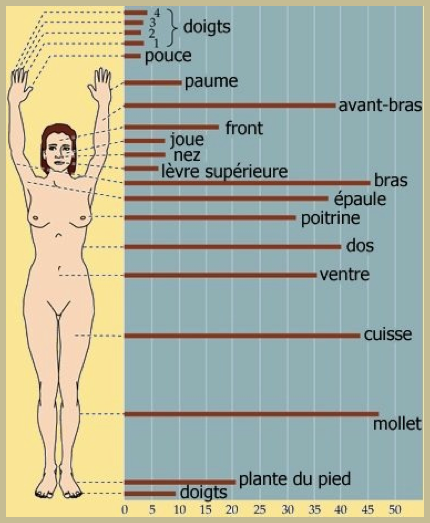
\includegraphics[width=10cm]{1_Bible/Photos/Biology/discrim_spatiale.png}
	\caption{Tests des deux points}\label{discrim_spatiale}
\end{figure}
Les parties les plus sensibles sont les mains, le visage et les doigts de pieds.

\subsection{Méthode de mesures psychophysique}
...

\subsubsection{Méthode classique}
...

\subsubsection{Théorie de la détection du signal}
...




